\newpage
\section{Wasserdargebot für Wasserkraft}

\subsection{Abflussganglinie}
Abfluss $Q_b$ in $\frac{m^3}{s}$ während eines Jahres (365 Tage)\\
\begin{minipage}[c]{0.58\columnwidth}
    \begin{center}
        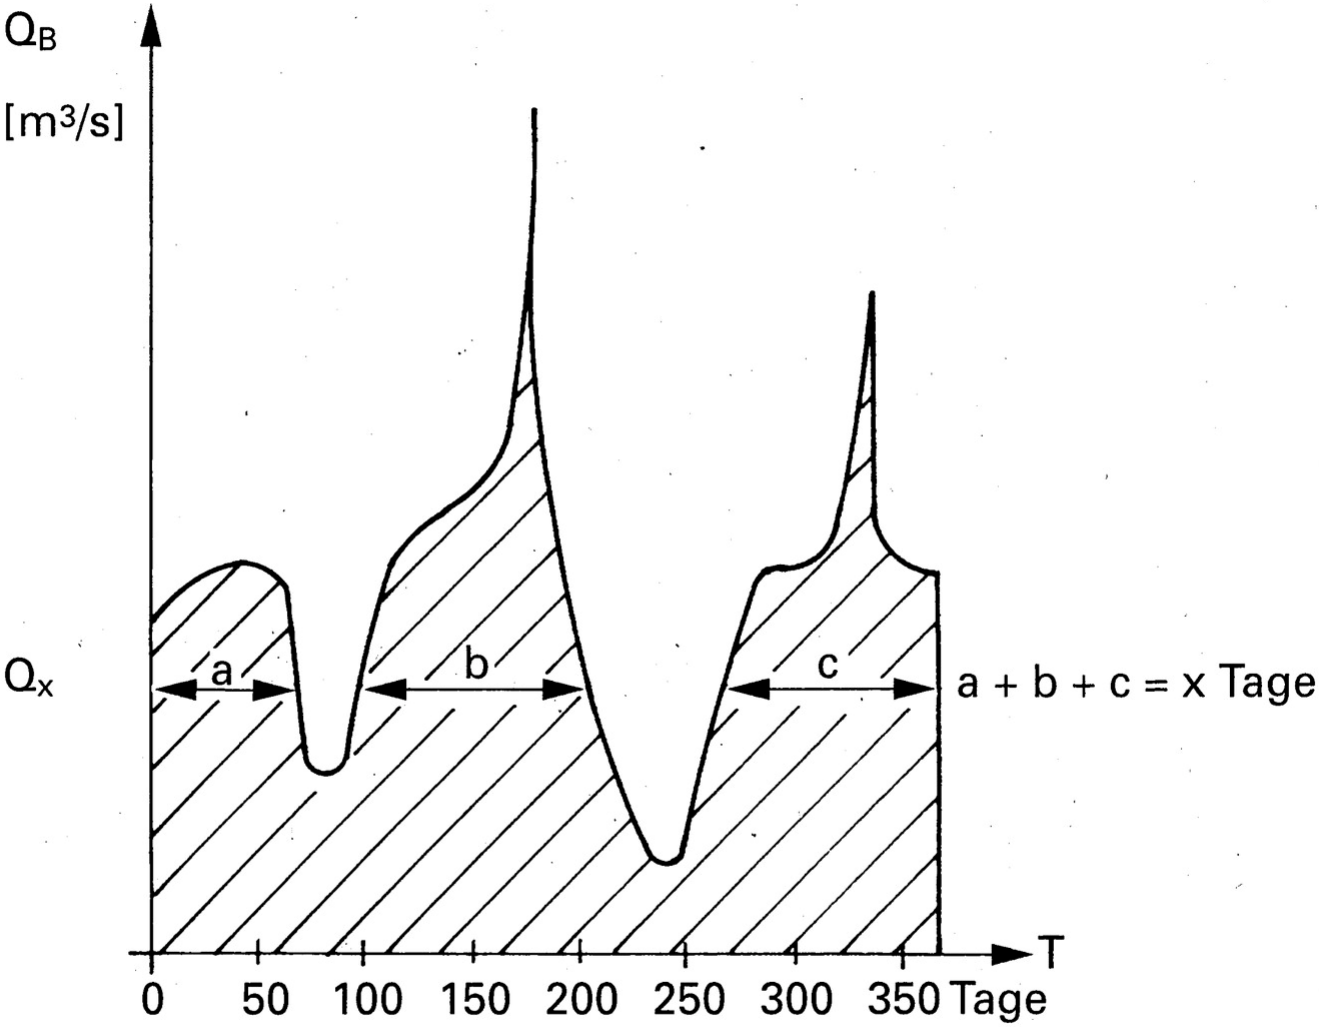
\includegraphics[width=0.95\textwidth, align=c]{images/Abflussganglinie.png}
    \end{center}
\end{minipage}

\vspace{0.25cm}



\subsection{Abflussdauerkurve}
Abfluss $Q_b$ in $\frac{m^3}{s}$ während eines Jahres (365 Tage), sortiert der Grösse nach\\
\begin{minipage}[c]{0.48\columnwidth}
    \begin{center}
        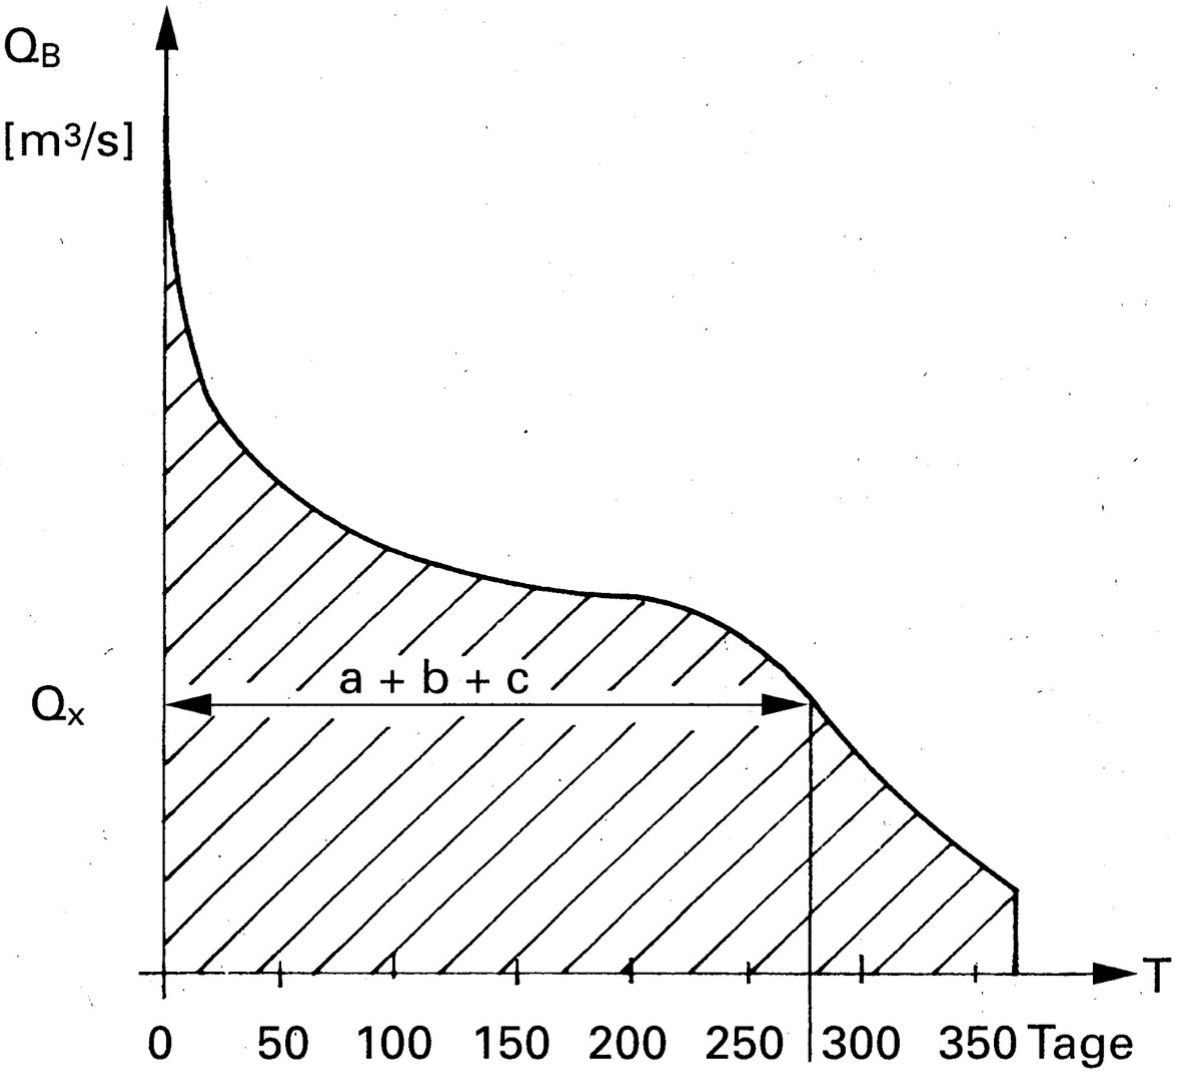
\includegraphics[width=0.95\textwidth, align=c]{images/Abflussdauerkurve.png}
    \end{center}
\end{minipage}

\vspace{0.25cm}

\textbf{Abfluss ist an 275 Tagen mindestens $Q_x$}



\subsection{Nutzwassermenge}
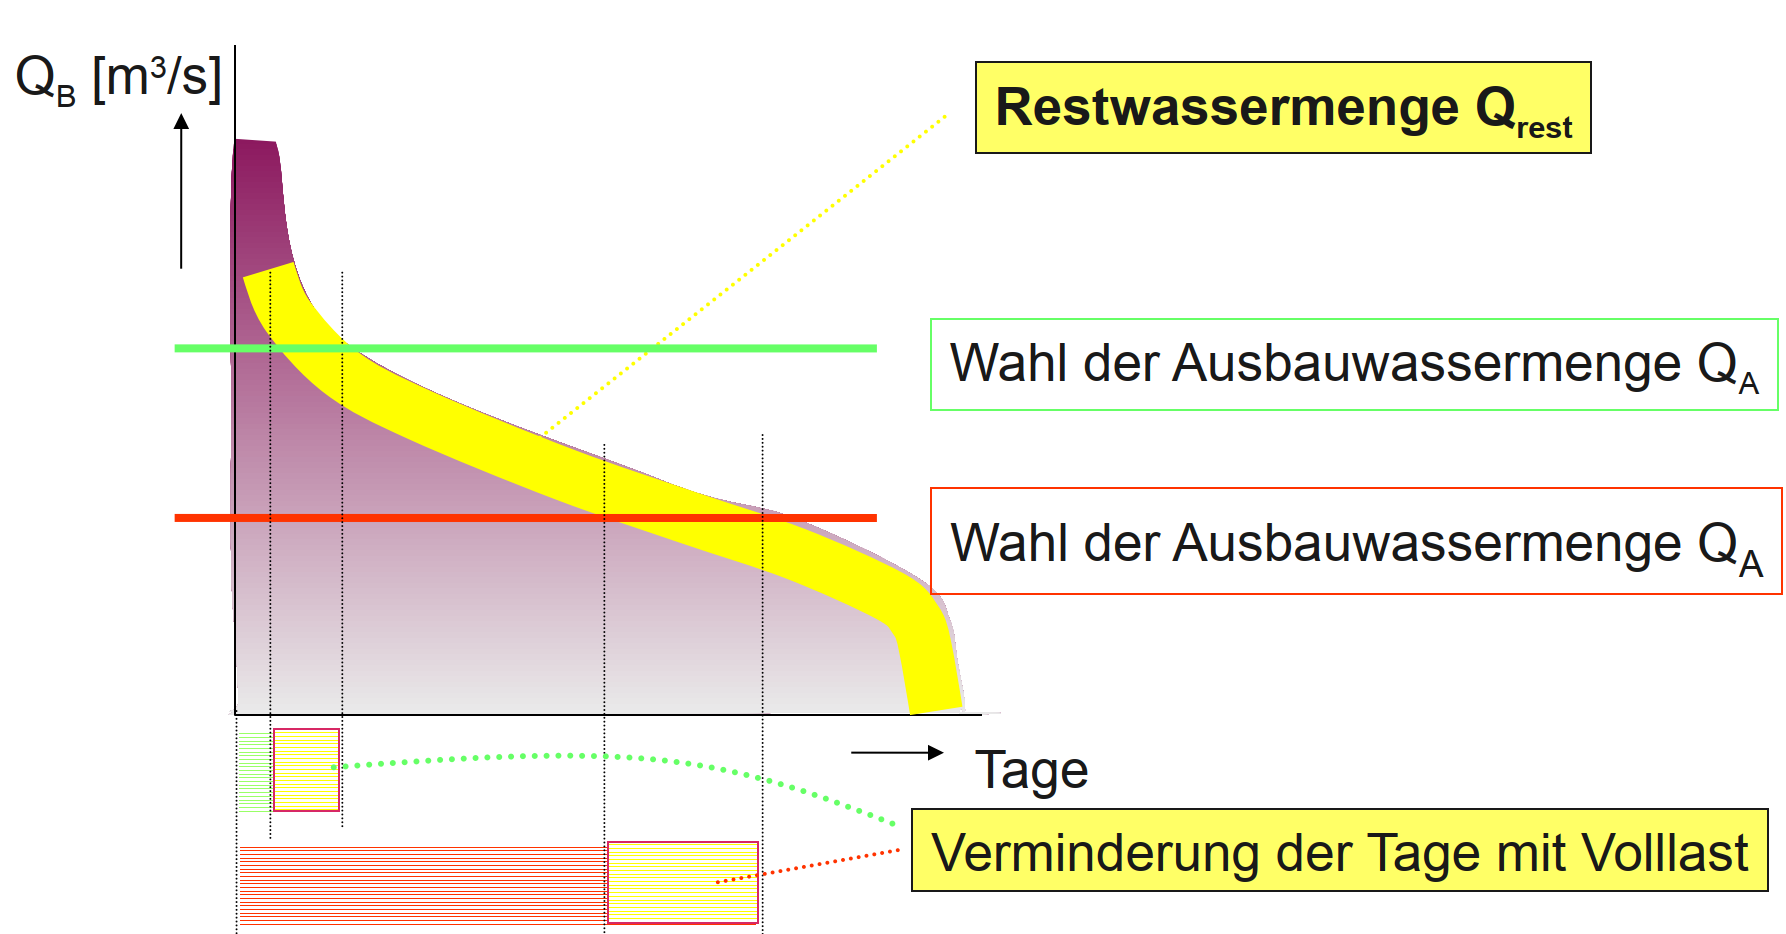
\includegraphics[width=0.95\columnwidth, align=c]{images/Nutzwassermenge.png}

\vspace{0.25cm}

$\boxed{Q_{Nutz} = Q_B - Q_{Rest}}$

\vspace{0.25cm}

\renewcommand{\arraystretch}{1.2} % Erhöht Zeilenhöhe für bessere Lesbarkeit
\begin{tabular}{@{} l p {6cm} l @{}}
    $[Q_{Nutz}]$    & Nutzwassermenge   \dotfill & $\frac{m^3}{s}$ \\
    $[Q_B]$         & Abflussmenge      \dotfill & $\frac{m^3}{s}$ \\
    $[Q_{Rest}]$    & Restwassermenge   \dotfill & $\frac{m^3}{s}$ \\
\end{tabular}















